\documentclass[10pt,conference]{IEEEtran}
\usepackage{cite}
\usepackage{amsmath,amssymb,amsfonts}
\usepackage{algorithmic}
\usepackage{graphicx}
\usepackage{textcomp}

\usepackage{booktabs}

\usepackage[table]{xcolor}
\usepackage{paralist}
\usepackage{url}

\usepackage{boxedminipage}
\usepackage{enumitem}
\usepackage{graphicx}  
\graphicspath{
	{figures/}
}
\DeclareGraphicsExtensions{.pdf,.jpeg,.png}


% Complex \xxx for making notes of things to do.  Use \xxx{...} for general
% notes, and \xxx[who]{...} if you want to blame someone in particular.
% Puts text in brackets and in bold font, and normally adds a marginpar
% with the text ``xxx'' so that it is easy to find.  On the other hand, if
% the comment is in a minipage, figure, or caption, the xxx goes in the text,
% because marginpars are not possible in these situations.
{\makeatletter
 \gdef\xxxmark{%
   \expandafter\ifx\csname @mpargs\endcsname\relax % in minipage?
     \expandafter\ifx\csname @captype\endcsname\relax % in figure/caption?
       \marginpar{\textcolor{red}{xxx~}}% not in a caption or minipage, can use marginpar
     \else
       \textcolor{red}{xxx~}% notice trailing space
     \fi
   \else
     \textcolor{red}{xxx~}% notice trailing space
   \fi}
 \gdef\xxx{\@ifnextchar[\xxx@lab\xxx@nolab}
 \long\gdef\xxx@lab[#1]#2{{\bf [\xxxmark \textcolor{red}{#2} ---{\sc #1}]}}
 \long\gdef\xxx@nolab#1{{\bf [\xxxmark \textcolor{red}{#1}]}}
 % This turns them off:
% \long\gdef\xxx@lab[#1]#2{}\long\gdef\xxx@nolab#1{}%
}


\title{ABC: Action-Based Test Carving}

\author{\IEEEauthorblockN{Alessio Gambi}
\IEEEauthorblockA{\textit{University of Passau} \\
%\textit{name of organization (of Aff.)}\\
Passau, Germany \\
alessio.gambi@uni-passau.de}%
}


\begin{document}

\maketitle

\begin{abstract}
\end{abstract}

\section{ABC}
\textbf{Overview}

Instrumentation:

We instrument application classes and test classes, but not system classes or supporting libraries. In particular we do not instrument JUnit libraries.
For this reason we cannot track the full execution of test setup actions (@Before), but rely on the user to list them during carving to include them, and
ensures that the state of the External environment is correctly setup before the execution of system tests (and later carved tests).
For example, if the application requires a working directory to exists, or files ot be in places, or a predefined content of the database, we ensure that.

Instrumentation is done by logging for each invocation, the method signature, parameters, owner instance (unless a method is static), and return value.
Informations about method signature and method owner are taken before method executions, return type after. This is to avoid losing informations when the application terminates by invoking system.exit (which prevents methods to return and us to collect return values and more importnatly ownership informations otherwise).

Instrumentation insert tracing calls, and XML Dumping calls such that informations about state of objects before and after a method invocations and informations about state of (non-primitives) return values are stored and available to create regression assertions (for delta debugging).

We track basic assignments of fields, string and array initialization, and array accesses as "artificial" invocations, such that we will uniform their treatment during carving which does not distinghuish between real and artifical method invocations anymore, hence simplifying the process.

System test execution and tracing:

We run the system tests with the instrumented code and produce a trace file containing the execution trace for each of them, as well as a set of xlm files which contain the serialized state of the objects used during the execution.

Carving:

Trace Parsing:

We parse the trace to create the following three main data structures for each system test (Figure + Example):
an execution flow graph which captures the temporal aspects, i.e., sequenciengn of the operations;
a call graph which captures the structural aspects, i.e., nesting /caller-calle dependenciens of the operations;
and, a data dependnecy graph which captures the data dependencies among the operations. Examples are ownership depednencies among an object instance and the methods called upon it, data dependencies on method parameters/arguments, and return values.

Carving is done in three logical steps: core carving, we carve the methods directly involved in the MUT; carving external interfaces, we carve methods that belongs to external interfaces, and finally,  including environment test setup. Carving steps are done conservatively by including all the calls that MIGHT influence the execution. This includes calls to CUT that precede MUT which might change its status, and calls to external interfaces that might change the status of the environemnt, for example, by creating or changing file or databased contents, or by login to external services, etc. 

Core carving: we start from the target MUT, and compute a backward slice by the computing the 
	intersection between the set of method invocations that happened BEFORE the target MUT, and the
	the method invocations which are reachable by means of data dependencies from the MUT. Those recursively include,
		all the calls which set up the CUT, and the calls which provide all the parameters of of the MUT.
	When it comes to providing parameters to functions, there might be two cases: the object is provided via its constructor and is modified by means of method calls, and the object is returned by another method calls. The latter for example is typical when application data are returned by Factory methods.
	To generate carve tests we consider all the possible combinations of these two cases for each parameter to the MUT, therefore we can create test cases like CODE1, where we completely disregards the application logic in favor of a direct constructions of dependencies, and like CODE2, where we rely on the actual code of the application under test to provide instances of required objects, as long as they correspond to behaviors observed during the execution of system tests.
	A final step, to avoid that by mix matching method invocations from different locations we end up calling the same methods multiple times, we use the call graph to compute subsumsion sets, that is, the set of method invoactions inside the carved tests, which are subsumed by method calls already included.
	This is illystrate in CODE 3. During this last step, it might happend that also the MUT is subseumed, thus removed, from the carved test.
	Since this violated the basic assumtpion of carved tests, that is, the MUT must be DIRECTLY called in the test, we reject those spurios tests.
	In theory, those tests are valid from the execution point of view, that is, the state of the application at the time the MUT is invoked is the correct one, 
	however, because of call nesting, there no easy (or any at all) way to extract the CUT and the return value of the MUT, making impossible to define correct assertions on them.
	\xxx{How do we handle the cases in which the same object, i.e., String buffer, is called multiple times? Do we take the last invocation or the one which is closer to MUT? If this becomes too complex. we might omit this details from the explanation.}

Algorithm ALGO summarize the action based test carving algorithm.

Carving of External interfaces (conservative): Users list the external interfaces upon which the SUT depends. Common interfaces include java.io.Files, java.nio.Paths which act as interface/api to the underlying File System, classed under java.sql which acts as interface to Sql databases, and java.util.Scanner, which act as interface to the user (via the Console/command line). We carve invocations on those external interfaces by recursively carving all the invocations to them which happens before MUT and which are NOT yet included in the CORE carving, to avoid calling external interfaces multiple times. For carving, we proceed similarly to Core carving \xxx{Double check the algorithm if we still consider combination of inputs}.

Including test setup methods (conservative): We do not instrument nor carve test setup methods, like the one commonly executed inside @Before.
The motivation here is that those methods configure the test environment for the system tests, i.e., they do not belong to the application logic,
but rather to system tests logic. Nevertheless, carving tests (might) require those methods to be in place. For example, a typical setup method drop and recreate the mysql database. This ensures that system tests start from a known state of the database. Since tests carved from the system tests rely on the same assumptions, we need to include and replicate the same setup before executing them. Again we adopt the conservative approach of including all the required setup calls to generate carving tests. This has the benefit to ensure that the right preconditions are in place, but has the drawback to increase the execution overhead of the carved test. Imagine the case a carved test performs a basic check on an input, i.e., the input shall be greater than 0. If this test was carve out of a system test which requires a databased filled with test data, our conservative approach will recreate the databased also for the carved test, unnecessarily. Because of this, we will proceed by minimizing the test cases and removing all the unnecessary method invocations from the carved test.


The last step is the actual test generation where we take carved and minimized tests are produce executable java (JUnit) tests. We use open source library to generate the java code from our internal representation based on jimple/soot.

\section{Evaluation}

\textbf{Goal of the evaluation} 

Show the usefulness of test carving by means of showing that 
carved tests stress the SUT in the same way systems test do, but at the unit level. 
That is we do not lose testing power/miss behaviors by using carved tests.
%
We illustrate this by showing how code coverage achieved by system and carved tests is the same.

Carve tests are more focused than system tests, hence, in a regression setting we do not necessarily need 
to execute all of them. This is not true in general for system tests which, by involving the entire system, end up in using (hence depending on)
all the system classes (or at least a great deal of it).
%
We illustrate this by modifying the system under test (using bogus, non-logic-modifing modificaitons) and counting how many system and carved
tests are executed after each modification. In particular, we show that modification of few classes already caused all system tests to be triggered,
while only a relevant subset of carved tests are re-executed.
%
\xxx{For the sake of completeness we show how execution time varies during regression, compared to fully re-executing all the carved tests?}

Delta debugging -> this one becomes part of the evaluation. Since we adopt a conservative approach to include all the calls which might be state chaging,
we are interesting to investigate if this is "a bad thing". How many of those actions are superfluous and can be safely removed?
This also gives us a hint on if/how it would be beneficial to use delta debugging to minimize the carved tests cases.

For doing so, we implemente a delta debugging appraoch to remove and test each action, and compare the results on execution time, coverage and regression test selection of original and minimized test to see.
	generate validation instruction based on XML serialized state. We do not literally compare the serialized state, because some objects cannot be serialized in a meaningful way (i.e., open data base connections, file descriptors, streams) and some objects are parameters of the tests and are injected as dependencies during testing. For example, temporary working dir, date objects relative to current date, and other data that are generated randomly at the beginning of each test (and never changed during the execution?). 
	
	\xxx{Give examples here on Employee and HotelReservation ? this means we need to introduce them as motivating scenarios?}
	
	Otherwise, we cannot remove dependencies correctly. \xxx{This requires an example}.
	We compare both the return value of the MUT if any, and the state of CUT.
	
	Starting from the instruction before MUT and going backwards, we remove one instruction, repeat the test execution, and check that the test passes. That is, no unhandled exceptions and no failed assertions.

	We assume a reset environment function, i.e., wipe out the database, is provided by the user to avoid polluting, and invalidating the result of delta debugging. Note that the carved tests instead do not require this, and are correct by design.
	
	\xxx{How much do we save in terms of instructions? and execution time?}

This is simple but effective solutions, however, it incurrs in a huge performance overhead because each carved test must be re-executed a number of times equals to the amount of instructions it contains. Optimization based on static analysis and data-flow analysis might be used here to identify cluster of invocations that belong together and possibly can be removed or left in the carved test all together. However, this is out of the scope of this paper and will be addressed in future work.
	\xxx{How much does it cost to run delta debugging?}

Benefits of Delta Debugging. Since delta debugging is expensive, we want to investigate/assess its cost/benefits. We do so by comparing execution time and number of instructions before and after minimization, as well as regression test selection.
%
Note that in this cases the evaluation is biased by the choice of the test subject, which do not involve external services (which might be slow and expensive to use), but only locally available resources.

\xxx{Maybe seel this thing of delta debugging as part of the evaluation to show that, because delta debugging does not remove many instructions, 
then the carved tests are already good, cannot be improved in that sense. Note that this accounts for the instructions not the method invocations executed !}

Overhead of carving.
We are also interested in assessing the overhead of the overall approach to derive conclusions on its practical applicability.
For this, we measure and report execution and slow down factors of instrumentation, tracing, carving, test generation, and delta debugging.

I suspect that delta debugging might shows benefits for those classes which do not involve or depend on external interfaces,
and are used frequently.
For example HotelView has barely no logic, but to test it there's a lot of setup that can be removed.
Really relevant?


\xxx{Carved tests are faster to execute than system tests.}
\xxx{Maybe we can show this per class under test: we need to execute only a subset of tests}
\xxx{With our test subjects, we cannot really shows this, since the time}

\subsection{Test Subjects}

Employee project.
Interactive command line utility to manage employee and salaries. It works by creating, reading, and deleting files.
\xxx{check if the same (or similar) to original carving work}
\xxx{Add stats?}

HotelReservation System project.
Interactive command line utility to handle an hotel reservation system. It uses mysql backend to manage the state of the applications.
\xxx{Add stats?}

\subsection{Experimental Settings}
System tests. The test subjects do not come with system tests, so I created them manually.
System tests work by resetting the state of the system before each test, mocking input commands, and cleaning up the state of the system
to avoid pollution~\cite{pollution}.
Additionally, system tests set up expectations on System.exit to avoid system and carved tests to abruptly halting the execution.

For the  Employee projects, I rely on temporary folders and predefined file contents.
For the HotelReservation, I rely on truncating the database and recreate it as expected (either empty, or with predefined content).

\xxx{How system tests are defined? Ideally I would like to create them by following a standard technique, in practice, I will motivate my choice
by saying I creating them to cover as much application state as possible, in a black box style.
That is, I consider "each" page of the application as state and navigate the application states by means of different input sequences.
The name should be coverage-transition? Check on the software testing class}

% Maybe a bit to verbose
To answer RQ1 and RQ2, I execute the system tests and measure the achieved coverage;
Next, I instrument the application,  repeat the execution of the same system tests to collect the trace, 
and from the trace carve the tests out. I generate carved tests and minimized carved tests using delta debugging.
Finally, I execute the carved and minimized carved tests to measure coverage, time to carve tests, 
time to generate tests, and time to minimize test via delta debugging.

To answer RQ3 I proceed as follow. 
Usefulness of Carve Tests:
I execute the Ekstazi tool~\cite{} on the original version of the code separately for system and carved tests.
Then, I randomly change a number of source files n (n={1, \ldots, N}, N is the total amount of application files (no tests, no Main)) in the project.
Next, I re-execute Ekstazi separately for ssytem and carved tests, but keeping the same modification , and collect information on how many system and carved tests where executed upon each modification.
Ekstazi will select only the tests which are needed to be re-execute to test the modification.
The modification is bogus, we do not modify for simplicity interfaces, but only implementation classes to avoid compilation problems.
We repeat the process for 20 times and for n from 1 to N (N is application classes)

\subsection{Results}

%\begin{table*}
%\centering
%\caption{Summary of Test Carving}
%\begin{tabular}{l l l l l l l l l}
%Project & System Tests &  Carved Tests & Class Coverage & Statement Coverage & Branch Coverage & time SYS &  time Carv &  time Carv MIN\\
%Employee & 7  & 87 &  100\% & 35\% & 14\%  & 0.045 & 0.081 & --\\
%Hotel Reservation & 5 & 145 & 100\% & 41 \% & 29\% & 0.615 & 7.78 & --\\
%\end{tabular}
%\end{table*}

\begin{table*}
\centering
\caption{Summary of Test Carving}
\begin{tabular}{l r r r r r r r r r r r}
\toprule
\multicolumn{1}{c}{Project} &
	\multicolumn{3}{c}{Tests} &
	\multicolumn{3}{c}{Stmt. Coverage} &
	\multicolumn{3}{c}{Branch Coverage} &
	\multicolumn{2}{c}{Time} \\
&
	\multicolumn{1}{c}{S} & \multicolumn{1}{c}{C} & \multicolumn{1}{c}{M} & 
	\multicolumn{1}{c}{S} & \multicolumn{1}{c}{C} & \multicolumn{1}{c}{M} &
	\multicolumn{1}{c}{S} & \multicolumn{1}{c}{C} & \multicolumn{1}{c}{M} &
	\multicolumn{1}{c}{Carving} & \multicolumn{1}{c}{Minimiz.}
	\\
\midrule % Size of trace 1136 5809
Employee & 7  & 89 & 89 & 34\% & 34\% & 30\% & 14\% & 14\% & 12\% & 11 & 1,011 \\
Hotel Reservation & 5 & 145 & 145 & 41\% & 41\% & 40\% & 29\% & 29\% & 28\% & 19 & 4,839 \\
\bottomrule
\end{tabular}

Size of carved test
	min	max mean
E	25 	98	56.57
H	17	184	90.06
	
Average Minimization for
	Employee: 60.88583 \%, 9 out of 89 where NOT minimized
	Hotel Me : 65.8468 \%, 8 out of 145 where NOT minimized


%Time: 7.362
%
%OK (128 tests)
%====================================
%parsingTime 1031
%carvingTime 6095
%testGenerationTime 7265
%minimizationTime 3609319
%====================================

\xxx{Repeat the analysis and that the average execution time}
\end{table*}

\begin{figure*}[t]
\centering
\begin{minipage}[b]{.45\textwidth}
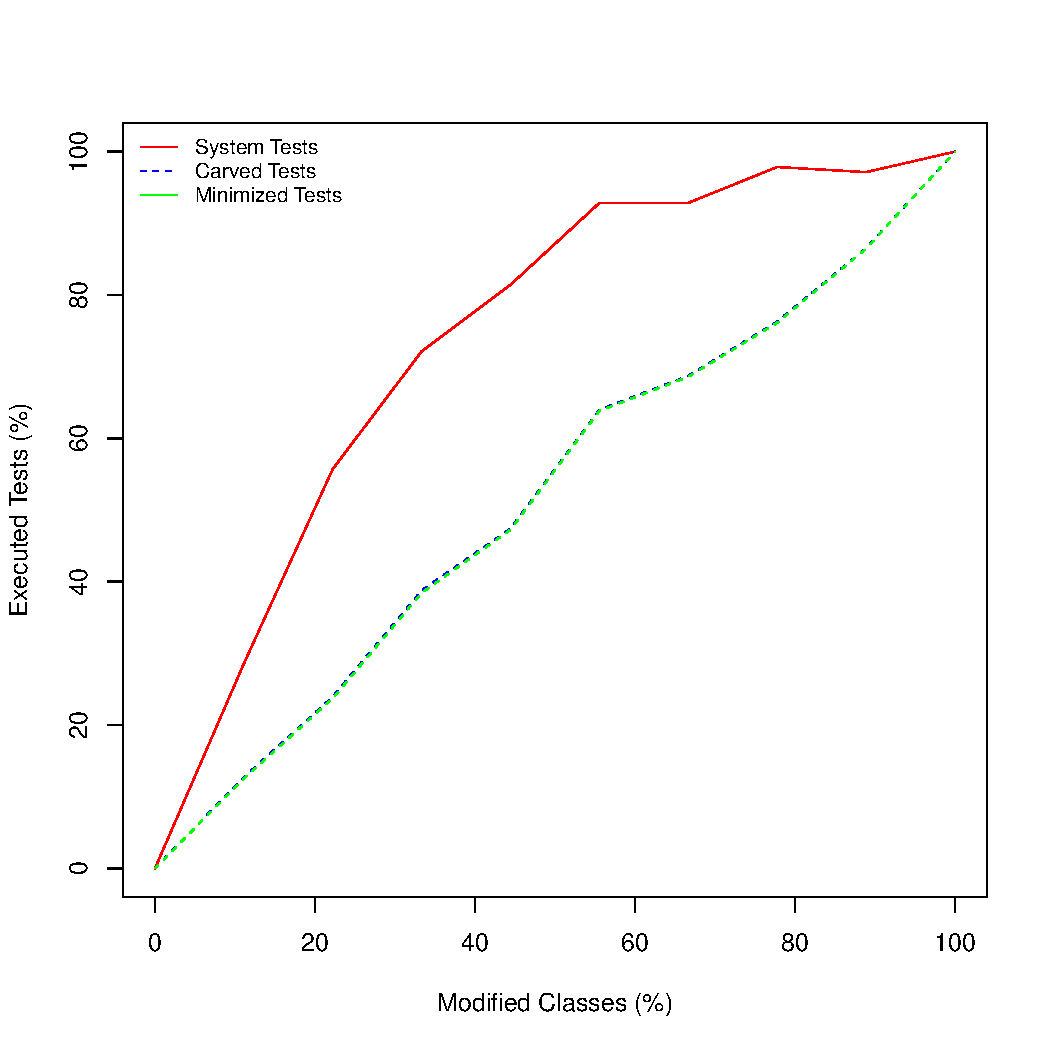
\includegraphics[width=\columnwidth]{figures/employee-rts-size}
\caption{Test Regression Selection - Employee}
\end{minipage}\hfill
\begin{minipage}[b]{.45\textwidth}
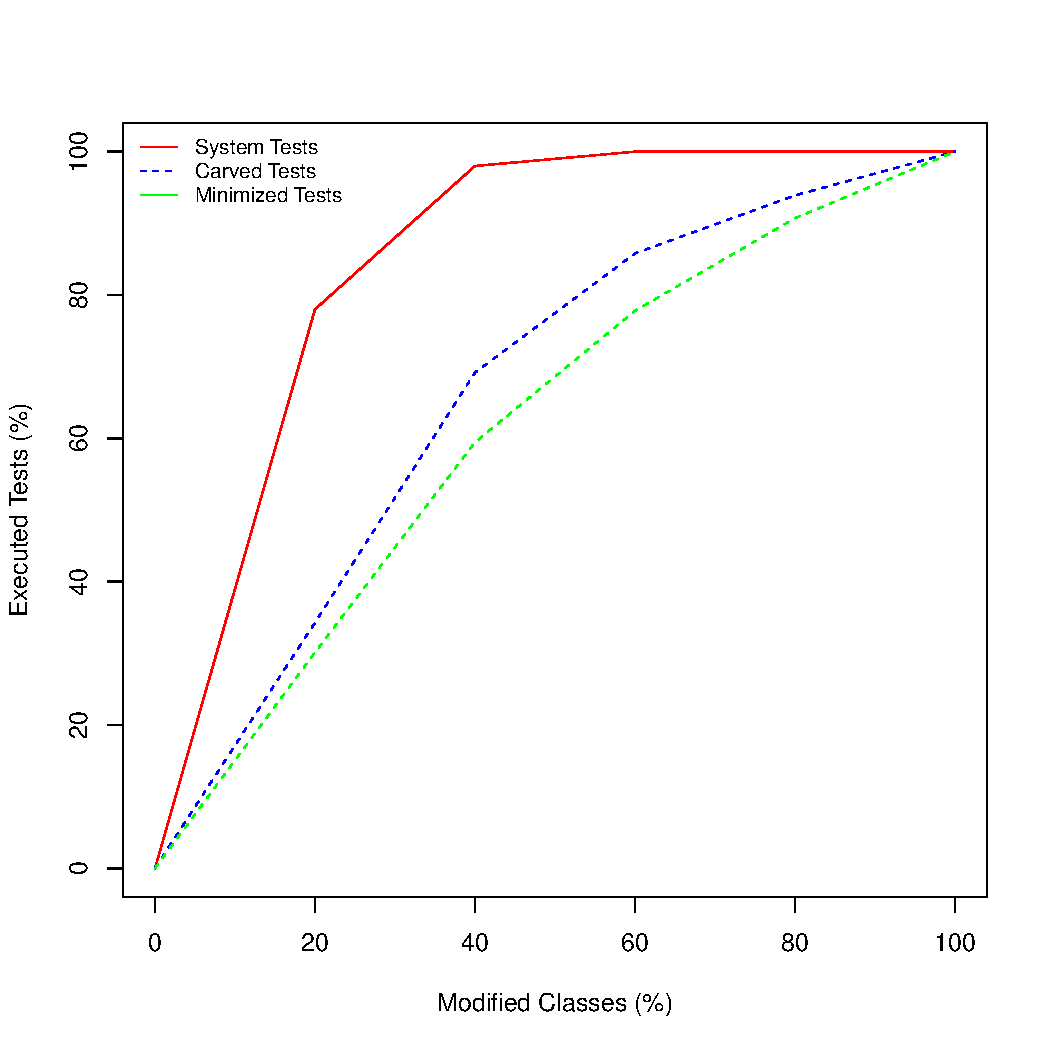
\includegraphics[width=\columnwidth]{figures/hotelme-rts-size}
\caption{Test Regression Selection - Hotel Reservation}
\end{minipage}
\end{figure*}


\begin{figure*}[t]
\centering
\begin{minipage}[b]{.45\textwidth}
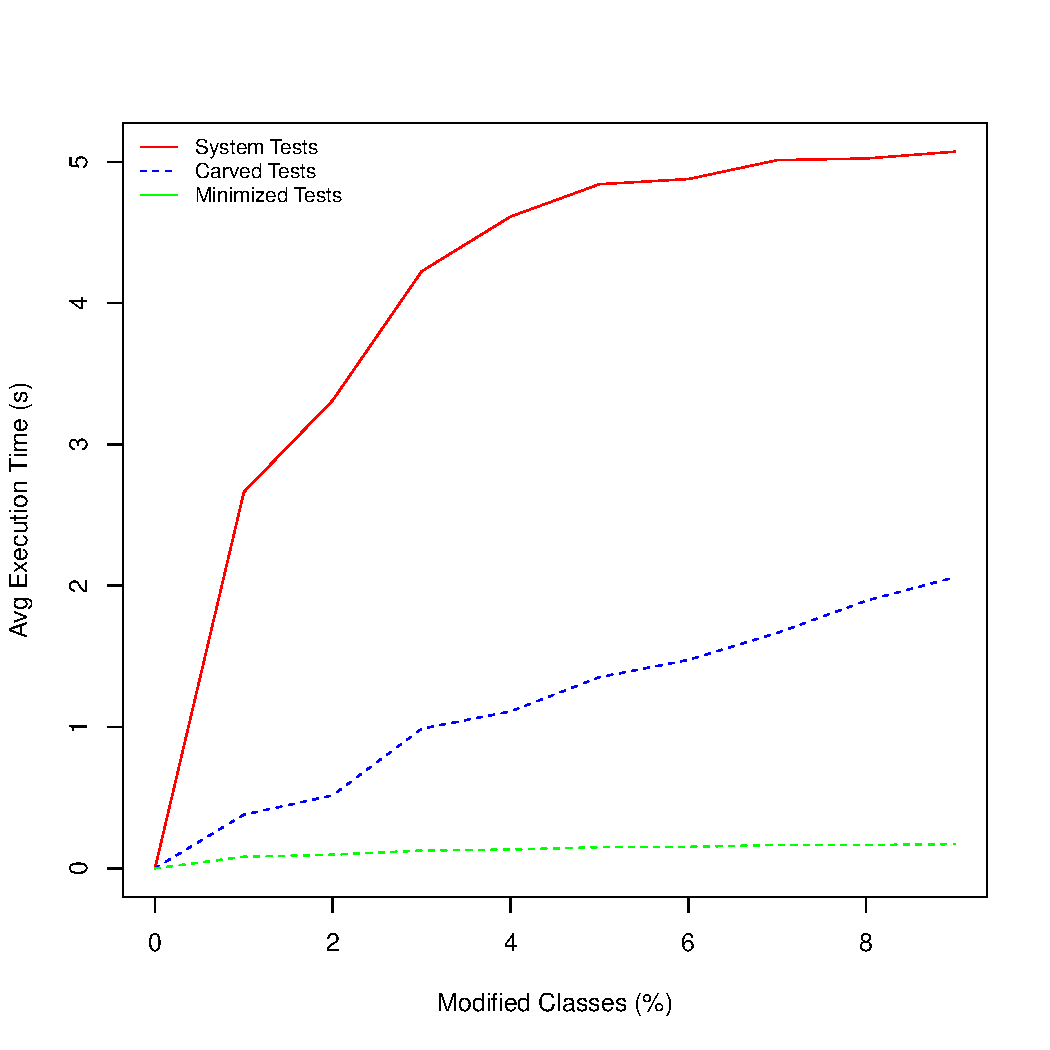
\includegraphics[width=\columnwidth]{figures/employee-rts-time}
\caption{Test Regression Selection - Execution time - Employee}
\xxx{Not sure this is relevant - update the system tests to last longer and explore more app behaviors}
\end{minipage}\hfill
\begin{minipage}[b]{.45\textwidth}
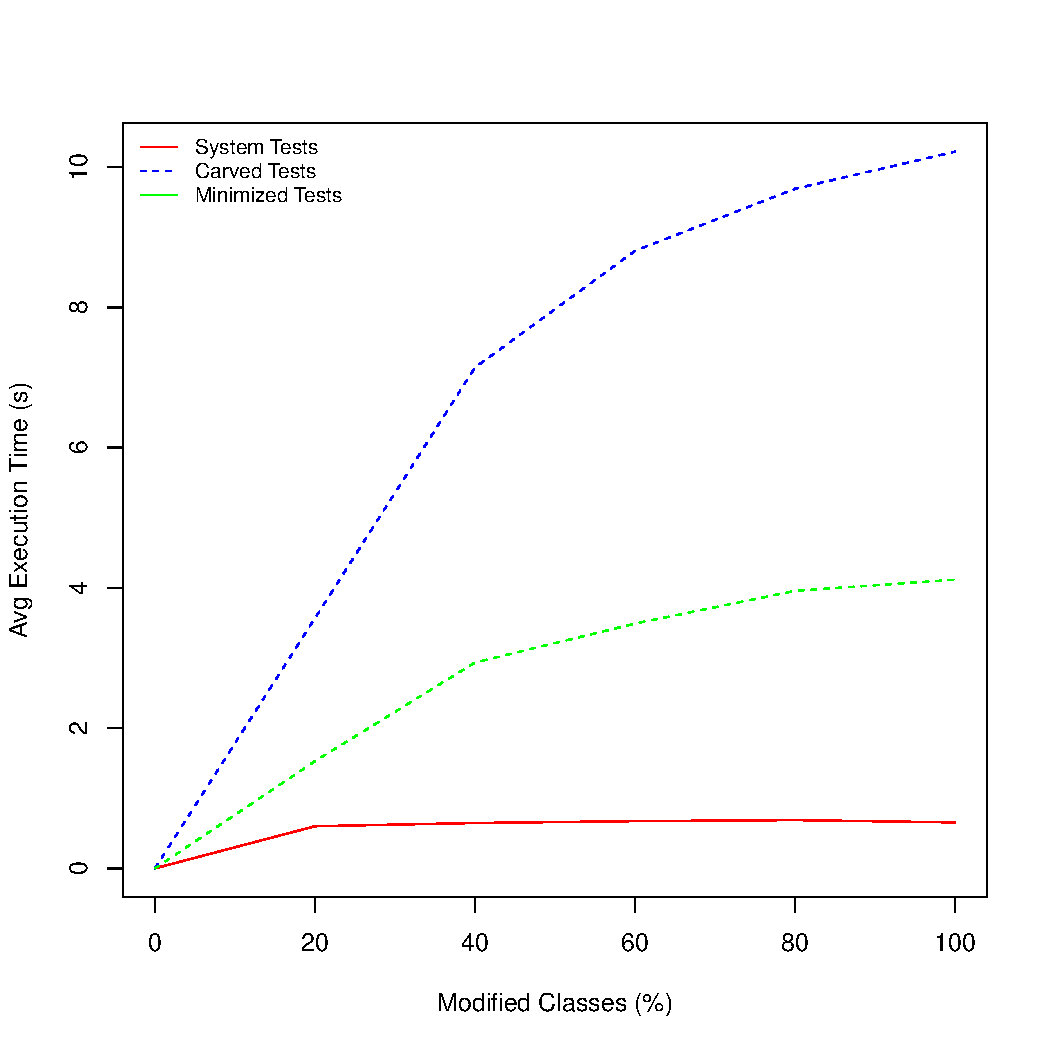
\includegraphics[width=\columnwidth]{figures/hotelme-rts-time}
\caption{Test Regression Selection  - Execution time -  Hotel Reservation}
\xxx{Not sure this is relevant - update the system tests to last longer and explore more app behaviors}
\end{minipage}
\end{figure*}

\subsection{Observation}
\xxx{For employee, Why the number of carved tests keep changing for hotel me?}
\xxx{For some }


\subsection{Discussion}
Coverage is the same

Execution time is larger for carved unit tests fro projects with simple setup.

We can generate tests for all the classes

Does minimization make sense?


Should I keep or not the test setup calls intact? Should I instead disassemble those as well ?!

Delta Debugging dominates the test generation time.
There's no difference in RST with and without minimized test cases.
For SOME REASON the minimized tests it takes more time to execute than the normal ones..
%
How many tests minimized? and how much?
%Employee: 87, 13 minimized (~14\%), those have an avg minimization of 95.55\%

% Is there a differnce in RTS.
Employee: there no difference in RTS, exactly the same tests are selected upon the same modifications.

\subsection{Limitations}
Action based carving need to "see" how object instances are created, otherwise might not be able to perform the carving because there's no way for the carver to reconstruct the object instance.

We observed this problem for example with test setup calls?

\subsection{Discussion}

Complex programs with GUI and WebApplications call for a hybrid approach: the hybrid approach provides (if possible) the parameters to the entry points of the application, for example, the servlet or the logic behind the GUI, which otherwise cannot observe the object creation thus replicate it.
With an hybrid approach, one might serialize the parameters of the calls and reload them to spin off the carving. E.g., one can define mocks that provide http requests, fill in with values objserved during the execution.

\end{document}